\chapter{An exciting observable}
\label{ch:nedm-at-psi}

% \begin{center}
%   \emph{The chief forms of beauty are order and symmetry and definiteness, which the mathematical sciences demonstrate in a special degree.}\\
%   Aristotle
% \end{center}


% \begin{center}
%   \emph{Why are we here? Because of CP-symmetry violation.}\\
%   prof. Edward Hinds
% \end{center}

\begin{flushright}{\slshape    
  The chief forms of beauty are order and symmetry and definiteness,\\
  which the mathematical sciences demonstrate in a special degree.} \\ \medskip
--- Aristotle
\end{flushright}

\bigskip

% \begin{flushright}{\slshape    
%   Why are we here?\\
%   Because of CP-symmetry violation.} \\ \medskip
% --- Prof.\ Edward Hinds
% \end{flushright}

% \bigskip

\section{Symmetries}

% Symmetry is the most fundamental form of beauty.

The essence of classical physics is the three symmetries: with respect to spatial translation (homogeneity of space), with respect to rotation (isotropy of space) and with respect to translation in time (homogeneity of time). As Noether showed, they correspond to the conservation laws of momentum, angular momentum and energy, respectively~\cite{Noether1918}. By saying a symmetry is conserved, we understand that no physical system becomes any different by \emph{only} having been moved in space, rotated, or looked at later.

These are continuous symmetries. No less fundamental is the triad of symmetries with respect to discrete transformations: $P$, parity transformation, mirroring the spatial dimensions; $T$, time reversal, flipping the arrow of time; and $C$, charge conjugation, flipping \emph{all} charges of particles. One would expect a beautiful universe to work exactly the same in a mirror, or with matter swapped with antimatter. This expectation is extended to combined symmetries, like $CP$, which flips the charges \emph{and} mirrors the space. The combined $CPT$-symmetry has a special place in physics, as it is obeyed by any Lorentz invariant local quantum field theory with a Hermitian Hamiltonian~\cite{Sachs1987}.
% It scares a humble experimental physicist to think of a theory which would not fulfill this.

\marginpar{Andrei Sakharov, pacifist and human-rights activist, was awarded the 1975 Nobel Piece Price and called ``a spokesman for the conscience of mankind''.}
Yet, in a perfectly symmetric universe after the Big Bang an equal amount of matter and antimatter would be created, and they would perfectly annihilate. Luckily, this did not happen, but the question \emph{why} remains one of the big unsolved problems in physics.
In 1967 Andrei Sakharov proposed, that the mechanism leading to the leftover matter  is based on a violation of the $CP$-symmetry~\cite{0038-5670-34-5-A08}.

Already a decade before, physicist have observed for the first time violations of one of the discrete symmetries in their laboratories.
In 1956 Chien-Shiung Wu shocked the physics world with her discovery of $P$ violation in beta decay of cobalt-60~\cite{PhysRev.105.1413}. Shortly thereafter, in 1964, the discovery of $CP$ violation in $K^0_L \rightarrow \pi^+ \pi^-$ decay left the physics world stunned again~\cite{PhysRevLett.13.138}. Now, both are explained in the scope of the Standard Model of particle physics. In the model the $CP$-violation appears in the weak sector as a complex phase in the Cabbibo--Kobayashi--Maskawa matrix, the matrix that mixes the mass and weak interaction eigenstates of quarks~\cite{doi:10.1143/PTP.49.652}.

$CP$ violation also appears in the strong sector of the Standard Model's quantum chromodynamics, as an additional term parametrised by $\theta_\text{QCD}$. Yet, no $CP$ violation in the strong sector has been observed so far. $\theta_\text{QCD}$, expected to be $\mathcal{O}(1)$, is limited to be smaller than \num{e-10}~\cite{PDG2016}. A puzzle in itself, this another unanswered problem in physics is referred to as the strong $CP$ problem.

All together, the degree of $CP$-symmetry violation in the Standard Model is not enough to explain the Universe we observe. The observed matter--antimatter asymmetry is around \num{e-10}, while only \num{e-18} can be attributed to the model~\cite{Riotto1999}. Despite the tremendous success of the Standard Model, we know it is not the full picture. We \emph{know} that the $CP$-symmetry is violated somewhere still, but do not know where or how~\cite{Pospelov2005}.%Naturally, we want to find out. 

Many theories beyond the Standard Model have been proposed that offer to solve this problem, among others. A very popular idea is to introduce additional particles around the scale of weak interactions (several-hundred GeV), as, for example, supersymmetry does~\cite{Supersymmetry}. Those theories typically introduce additional mechanisms of $CP$-violation, which provide an opportunity to test their prediction~\cite{Ellis1989}.



\section{Electric Dipole Moments}
Electric dipole moments (EDMs) are excellent probes for physics beyond the Standard Model~\cite{Pospelov2005}. An EDM is a $T$-violating, and assuming the $CPT$ conservation, also $CP$-violating observable. In a non-relativistic case of a particle in an electric and magnetic field, with the magnetic and electric moments $\mu$ and $d$, the Hamiltonian is
\begin{equation}
  H = - \mu \, \mathbf{B} \cdot \frac{\mathbf{S}}{S} - d \, \mathbf{E} \cdot \frac{\mathbf{S}}{S} \ .
\end{equation}
For a spin $S = \tfrac{1}{2}$ particle:
\begin{equation}
  H = - 2 \left( \mu \, \mathbf{B} + d \, \mathbf{E} \right ) \cdot \mathbf{S} \ .
\end{equation}
Vectors, like $\mathbf{E}$, are $P$-odd, while pseudovectors, $\mathbf{B}$ and $\mathbf{S}$, are $P$-even. The Hamiltonian as whole is $P$-violating:
\begin{equation}
  H_P = - 2 \left( \mu \, \mathbf{B} - d \, \mathbf{E} \right ) \cdot \mathbf{S} \neq H \ .
\end{equation}
Under time symmetry the spin is reversed and so is the magnetic field, rendering the Hamiltonian $T$-violating:
\marginpar{Magnetic fields are produced either by magnetic moments, which flip under $T$ together with spins, or by a movement of charges, which also is reversed under $T$.}
\begin{equation}
  H_T = H_{CP} = + 2 \left( - \mu \, \mathbf{B} + d \, \mathbf{E} \right ) \cdot \mathbf{S} = - 2 \left( \mu \, \mathbf{B} - d \, \mathbf{E} \right ) \cdot \mathbf{S} \neq H \ .
\end{equation}
Note how in both cases setting $d = 0$ restores the symmetry.

EDMs are measured mainly in three kinds of systems.
Firstly, beams of cold paramagnetic molecules, like ThO and YbF, provide a great sensitivity to the EDM of the electron~\cite{ThO_eEDM,Hudson2011}.
Secondly, measurements of vapours of diamagnetic atoms, notably $^{199}$Hg~\cite{PhysRevLett.116.161601}, are the most sensitive EDM measurements.
Finally, the electric dipole moment of a free neutron, nEDM, is the topic of this chapter.
While the Standard Model predicts the nEDM to be below \SI{e-30}{\elementarycharge\centi\meter}, its extensions foresee it to be
% \SIrange[range-phrase=--,range-units=single]{e-29}{e-22}{\elementarycharge\centi\meter}. 
% as large as \SI{e-22}{\elementarycharge\centi\meter}.~\cite{Ellis1989}
larger~\cite{Ellis1989}. Measurements of the nEDM provide an opportunity to validate, or falsify, those theoretical models.
Also, the neutron EDM, provides (together with the EDM of ${}^{199}$Hg~\cite{PhysRevLett.116.161601}) the most sensitive handle on measurement of the $\theta_\text{QCD}$, parametrising the strong $CP$ problem~\cite{PDG2016}.



\section{Measurements of the nEDM}

\begin{figure}
  \centering
  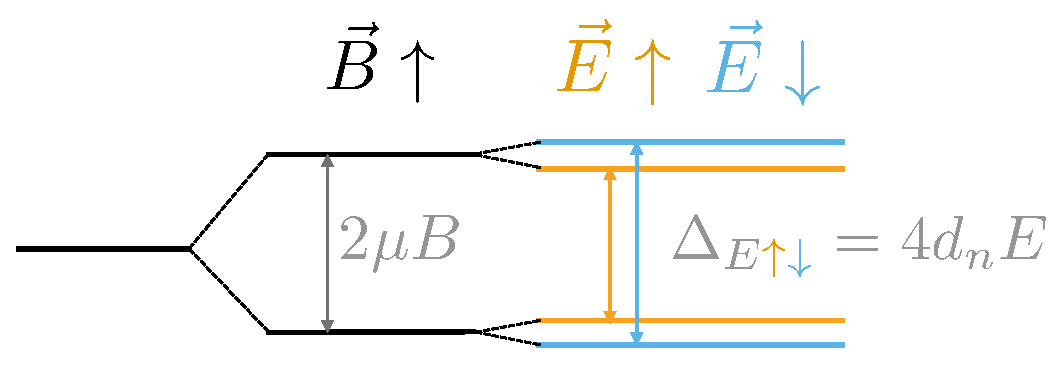
\includegraphics[width=0.7\linewidth]{gfx/introduction/measurement_principle.pdf}
  \caption{The energy states of a neutron in a combination of a magnetic and an electric field. The Hamiltonian is $H = - 2 \left( \mu_\text{n} \, \mathbf{B} + d_\text{n} \, \mathbf{E} \right ) \cdot \mathbf{S}$. The first term causes the first splitting of $2\mu_\text{n} B$. The second term increases or decreases, for the electric field parallel and antiparallel to the magnetic one respectively, the splitting by $2 d_\text{n} E$.}\label{fig:nEDM_measurement_principle}
\end{figure}

Already in 1950, before Wu's discovery of $P$-violation in the weak sector, Smith, Purcell and Ramsey proposed a measurement to test $P$-violation in the strong sector using the nEDM as the probe~\cite{PhysRev.78.807}. Their result, published in 1957, was consistent with zero $d_n = (-0.1 \pm 2.4) \times 10^{-20}\,\si{\elementarycharge\centi\meter}$~\cite{PhysRev.108.120}.

Figure~\ref{fig:nEDM_measurement_principle} illustrates the energy of a neutron in a magnetic field $B$, where it has two energy states separated by $2 \mu_\text{n} B$. The apparatus of Smith, Purcell and Ramsey could measure this separation, as a frequency, very precisely. In addition to the magnetic field, there was an electric one, either parallel or antiparallel to it. If there had been an nEDM, the energy separation would have increased in one configuration and decreased in the other. The difference between the energy separations measured in the two field configurations is proportional to the nEDM $d_\text{n}$.

\begin{figure}
  \centering
  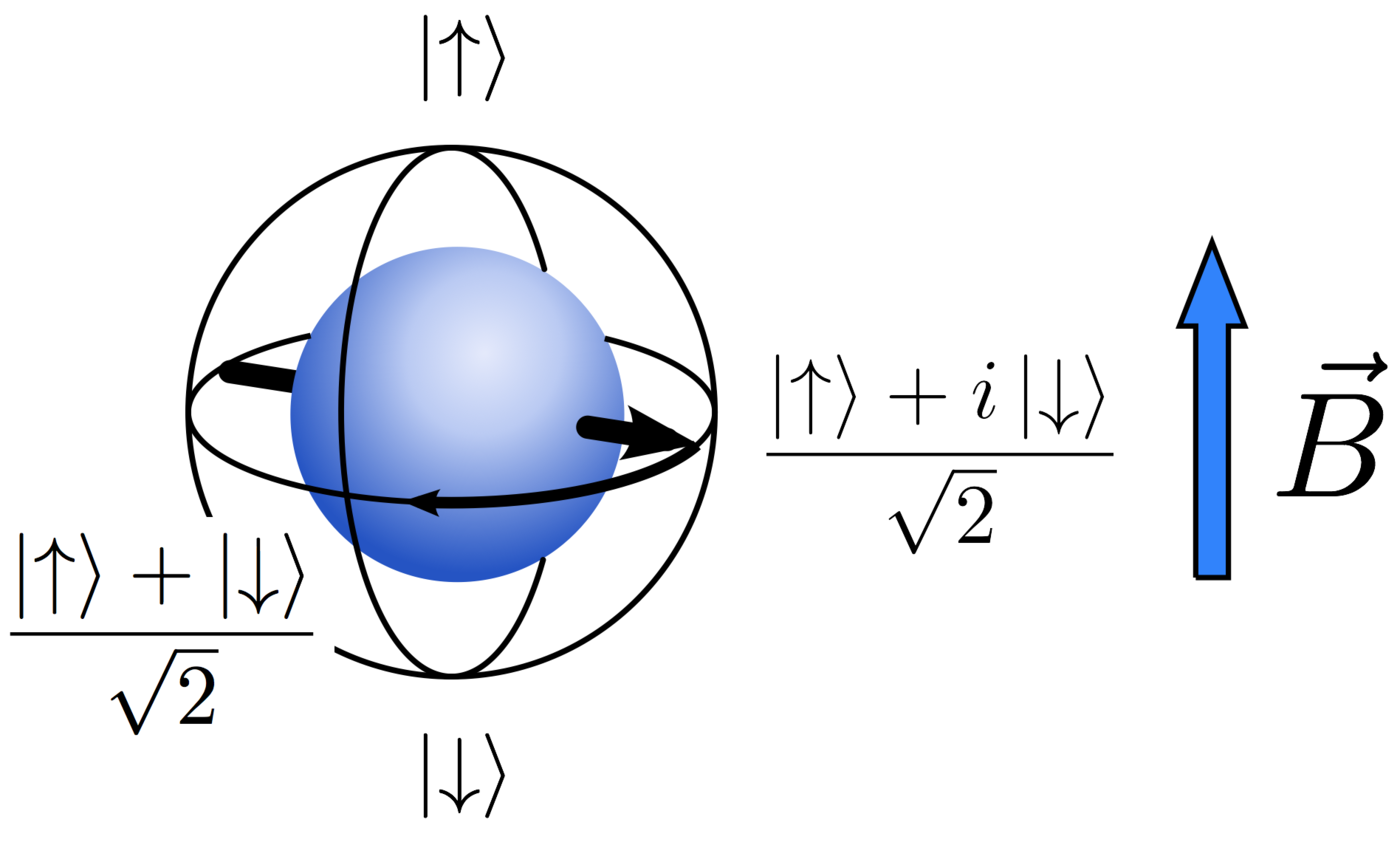
\includegraphics[width=.6\linewidth]{gfx/nEDMatPSI/bloch_sphere.png}
  \caption{A spin $1/2$ particle in a magnetic field on a Bloch sphere. The poles correspond to the pure spin-up and spin-down states. On the equator lie the states with an equal contribution of the two and the longitude corresponding to the quantum phase.}\label{fig:nEDM_bloch_sphere}
\end{figure}

To measure the energy separation between the two spin states they used what is now called the Ramsey method of separated oscillatory fields~\cite{PhysRev.76.996}. In order to explain it, let us first consider a neutron in a magnetic field, as pictured in Fig.\,\ref{fig:nEDM_bloch_sphere}. The neutron's spin is depicted there on the Bloch sphere, where the poles correspond to the pure spin-up and spin-down states. On the equator lie the states with equal content of the two, the longitude marking the quantum phase. When the spin state is not vertical, the interaction between the magnetic moment and the magnetic field causes the phase to spin. The frequency of the motion, called the Larmor precession, is proportional to the energy difference between the two states.
% \note{Maybe don't mix classical and quantum pictures.}

\begin{SCfigure}
  \centering
  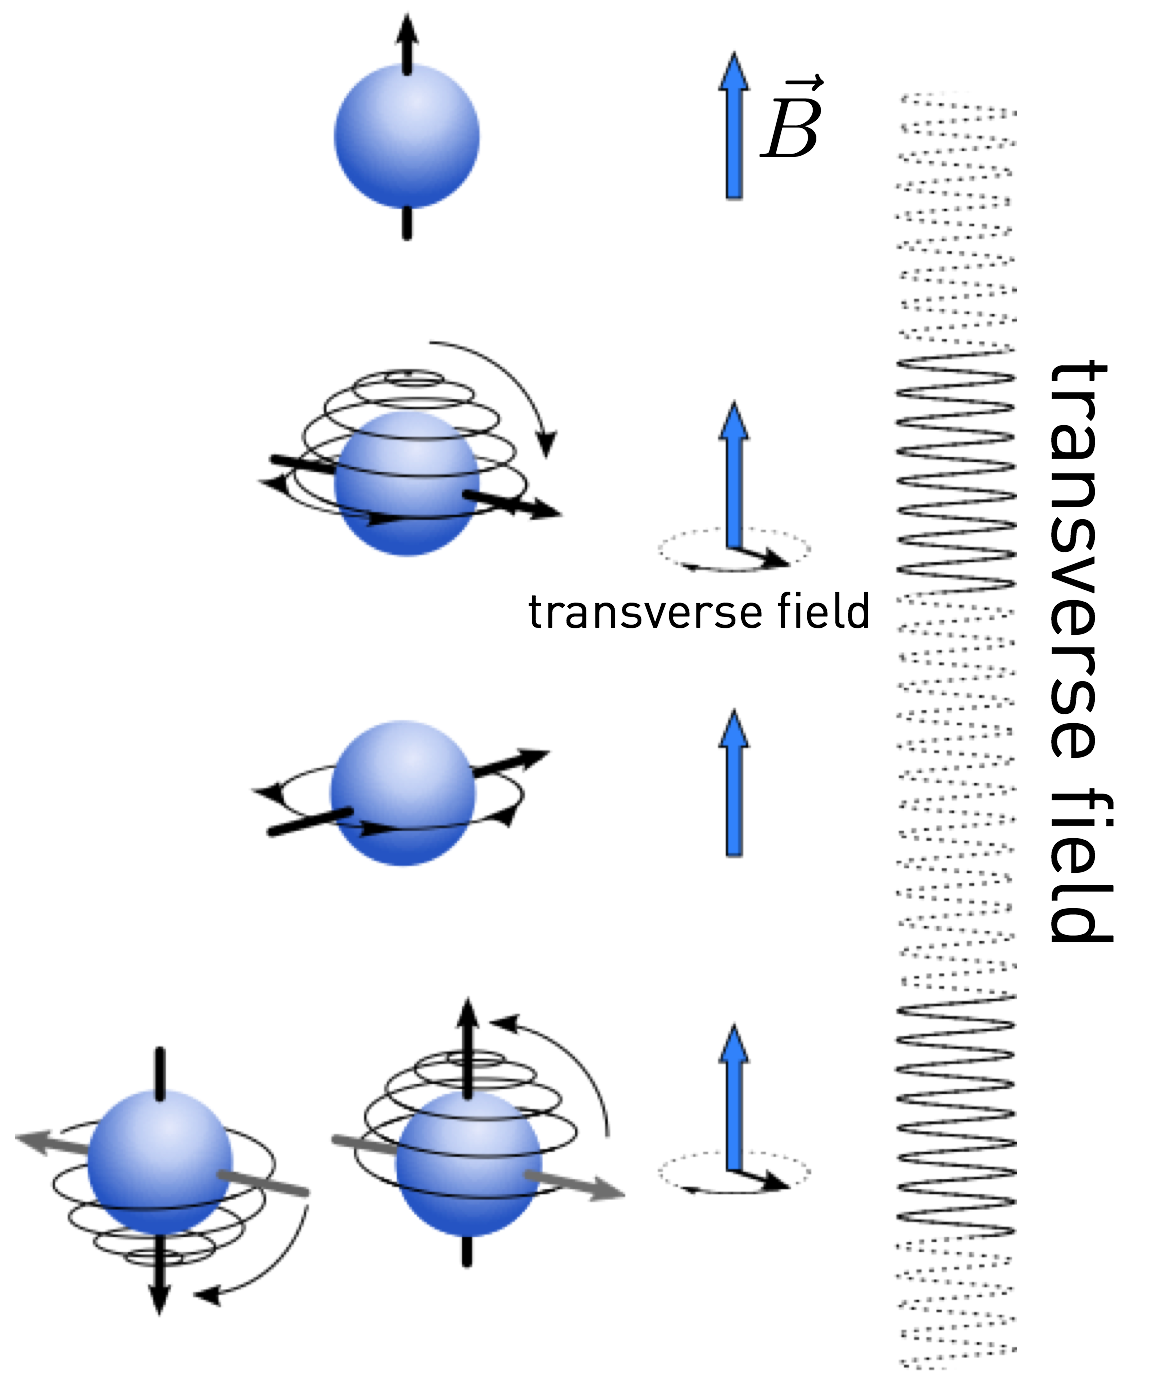
\includegraphics[width=.6\linewidth]{gfx/nEDMatPSI/Ramsey_principle.png}
  \caption{The principle of the Ramsey method, explained with the spin on the Bloch sphere. A polarised spin ensemble is in a magnetic field. A pulse of an oscillating transverse field flips the polarisation into the horizontal plane. The spin is allowed to freely precess in the field. Then, a second pulse of a transverse field is applied, in phase with the first one. The direction of the polarisation's flip depends on the relative phase between the spin and the transverse field.}\label{fig:nEDM_Ramsey_principle}
\end{SCfigure}

\begin{figure}
  \centering
  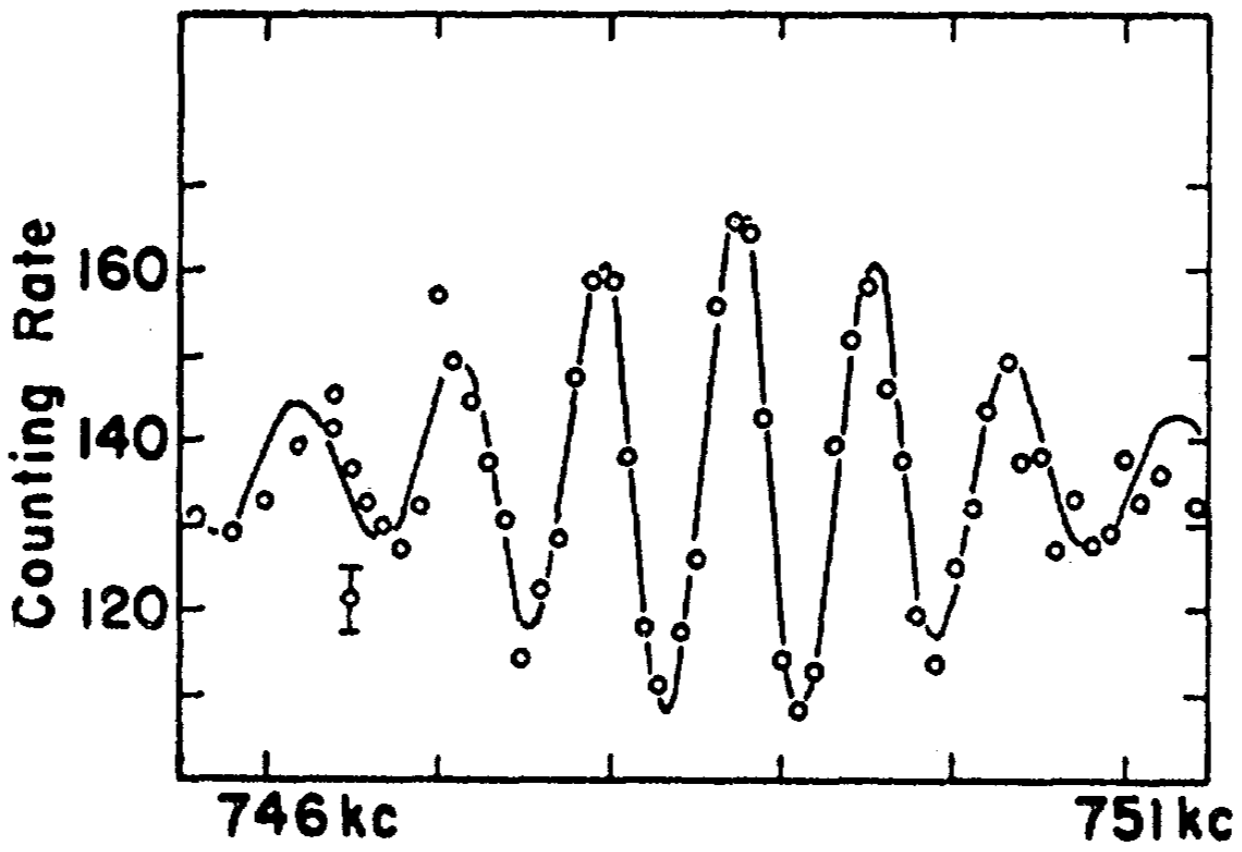
\includegraphics[width=.6\linewidth]{gfx/introduction/Ramsey_original_resonance.png}
  \caption{The original resonance curve measured by Ramsey~\cite{PhysRev.108.120}, showing the counting rate versus the frequency of the generator powering the spin-flipping coils.
  % The fringes are due the interference between the precessing spins and the transverse field.
  The width of the fringes is the inverse duration of the free precession. The envelope arises, as at a large detuning the spins were not flipped into the horizontal plane anymore.}\label{fig:nEDM_Ramsey_original_curve}
\end{figure}

In the experiment a nearly monochromatic neutron beam passed through a polariser, a region with an electric field, an analyser, and hit a neutron counter at the end. The whole setup was in a magnetic field. At the beginning and the end of the region with the electric field, there were coils producing an oscillating magnetic field in the direction perpendicular to the main magnetic field. The spin evolution between the two coils is depicted in Fig.\,\ref{fig:nEDM_Ramsey_principle}. When a neutron precessing in a magnetic field feels an additional oscillating field, transverse to the main one and of frequency close to the Larmor one, its spin undergoes a nutation---the precession plane moves along the main field (North or South on the Bloch sphere). The direction is determined by the relative phase between the spin's precession and the transverse oscillating field. In Ramsey's experiment the length of the coils was set to flip the neutrons' spins by $\pi/2$, so that after having passed the first coil they were precessing on the Bloch sphere's equator. The direction of the nutation in the second coil, and with it the probability of passing the analyser, depended on the relative phase between the precession and the transverse field. A slight change in the frequency of the generator powering the coils caused a considerable change in the phase difference that built up while the neutrons flew precessing between the coils. Scanning the frequency of the generator and monitoring the counting rate produced a resonance curve (Fig.\,\ref{fig:nEDM_Ramsey_original_curve}). The middle of the central fringe is the resonance frequency corresponding to the transition energy between spin-up and spin-down states.
% \marginpar{In the LNPI measurements slightly differ from Ramsey's technique. Instead of spin-flips, they used an adiabatic transition in inhomogeneous magnetic field, in order to account for different storage times of individual neutrons freely travelling through the bottle.}
Comparing the positions of the resonance with the magnetic and electric fields parallel and antiparallel gave the $d_n$ estimate.

\begin{figure}
  \centering
  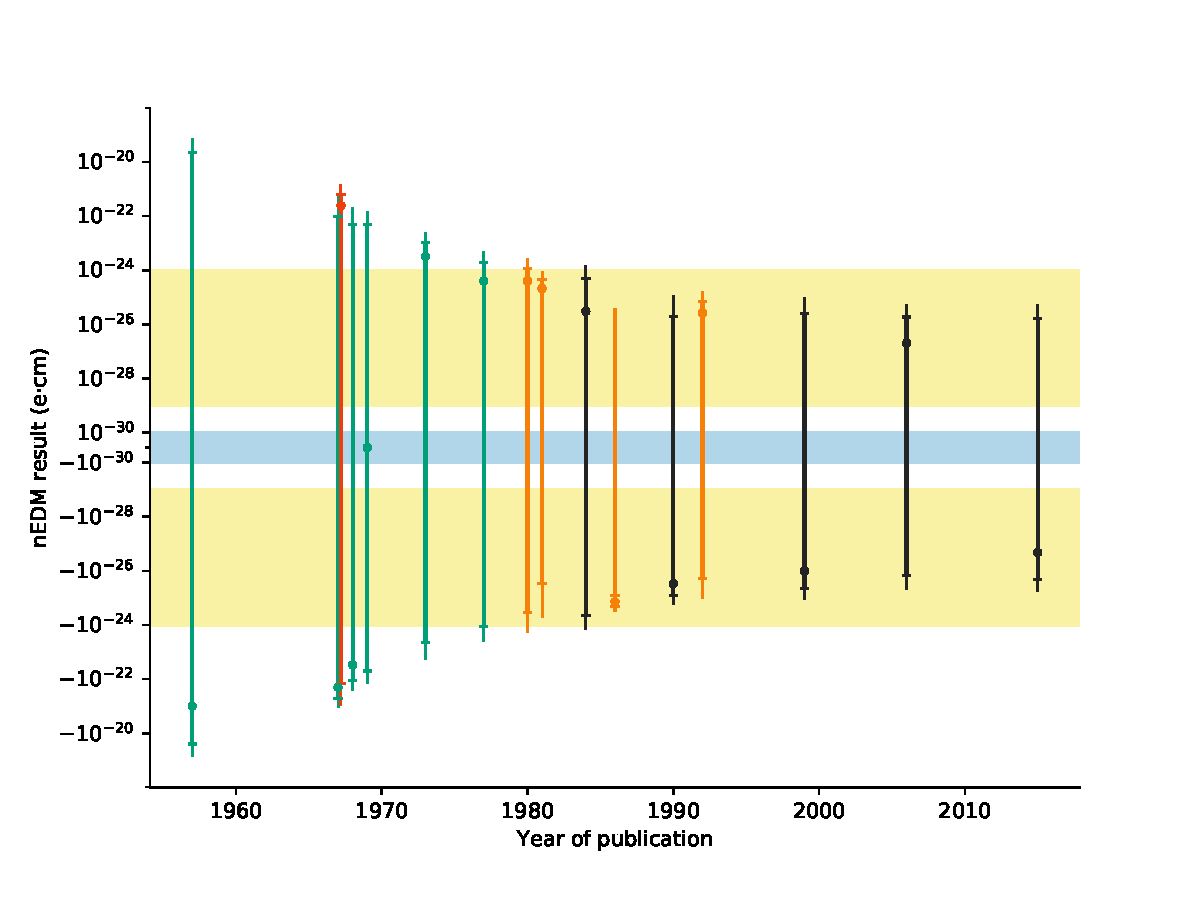
\includegraphics[width=\linewidth]{gfx/introduction/edm_limits.pdf}
  \caption{The history of the neutron electric dipole moment measurements. For each published result the vertical line corresponds to the $3\upsigma$ allowed region, horizontal bars depict the $1\upsigma$ one. The data markers are located at the central values of the measurements. The vertical scale is a combination of two logarithmic ones---one for each sign of nEDM\@. The region of the Standard Model's prediction is depicted in blue, the one of the proposed Model's extensions in yellow. The red line indicates a result obtained from a neutron scattering experiment. The sources are, in chronological order:~\cite{PhysRev.108.120,PhysRevLett.19.381,PhysRevLett.19.384,PhysRev.170.1200,PhysRev.179.1285,PhysRevD.7.3147,PhysRevD.15.9,ALTAREV1980269,ALTAREV198113,altarev1986search,ALTAREV1992242,PENDLEBURY1984327,SMITH1990191,PhysRevLett.82.904,PhysRevLett.97.131801,Pendlebury2015}}\label{fig:nEDM_limits_history}
\end{figure}

The community uses this technique to measure the nEDM until this day, their ever-more-sensitive efforts summarised in Fig.\,\ref{fig:nEDM_limits_history}. Until the 1970s the measurements were done using a beam of cold neutrons (marked in green), after then storage experiments greatly improved the time of the free precession and thereby the sensitivity. It was made possible by neutrons with kinetic energies below approximately \SI{300}{\nano\electronvolt} (referred to as ultracold), which are storable in some materials, by undergoing a total internal reflection~\cite{UCNbook}. In 1980 in the Leningrad Nuclear Physics Institute (LNPI, former USSR) the first measurement was performed with the neutrons being stored in a bottle~\cite{ALTAREV1980269}. The measurements in LNPI continued (orange) and in 1984 were joined by an international effort in the Institute Laue--Langevin in France (black).

A next effort took place in the Paul Scherrer Institute (PSI) in Villigen, Switzerland.
% In 2007 a new effort has begun in the Paul Scherrer Institute (PSI) in Villigen, Switzerland.
The experiment collected data over the years 2015--17 and at the time of writing the result was still being evaluated.
In the next chapter the nEDM measurement at PSI is described.
It serves as an introduction to the main part of this work, the original work of the author, which focuses on two aspects closely related to all nEDM measurements: stabilisation of magnetic fields and exotic physics that can be explored with those highly sensitive experiments.



\section{Magnetic stability}
The quality of the magnetic field is the main challenge in the measurements of the nEDM\@. Recall the principle of the measurement, as depicted in Fig.\,\ref{fig:nEDM_measurement_principle}. The electric dipole moment $d_\text{n}$ is proportional to the difference in the measured energy separations between the field configurations. Let us ask ourselves the following question: How big is a change in the magnetic field that causes a comparable change in the separation of the states?

The current nEDM limit is around $|d_\text{n}| < \SI{e-26}{\elementarycharge\centi\meter}$~\cite{PhysRevLett.97.131801}. Taking the electric field to be $\frac{ \SI{132}{\kilo\volt} }{ \SI{12}{\centi\meter} }$, as in the PSI experiment, this corresponds to an energy difference
\begin{equation}
  \Delta_{E\uparrow\downarrow} = 4 d_\text{n} E = \SI{4e-26}{\elementarycharge\centi\meter} \ \frac{ \SI{132}{\kilo\volt} }{ \SI{12}{\centi\meter} } = \SI{4.4e-22}{\electronvolt} \ .
\end{equation}
With the approximate neutron magnetic dipole moment~\cite{Green1982}
\begin{equation}
  \mu_\text{n} = \SI{-9.7e-27}{\joule\per\tesla} = \SI{-6e-8}{\electronvolt\per\tesla} \ ,
\end{equation}
the size of a change in magnetic field corresponding to this energy is
\begin{equation}
  \frac{ \Delta_{E\uparrow\downarrow} }{2 \mu_n} = \SI{3.7e-15}{\tesla} = \SI{3.7}{\femto\tesla} \ .
\end{equation}
\marginpar{In reality the requirement is relaxed by a factor of 10--100, as the final measurement is an average of several thousand measurements.}
This is about the strength of the magnetic field of a car passing several kilometers away. The field needs to be controlled on this level so that the two measurements, with the magnetic and electric fields parallel and antiparallel, can be subtracted from one another without the difference being dominated by the instability of the magnetic field.
% Even in the most quiet of nights the magnetic field at the experimental site was not more stable than about a nanotesla, and during a day the variations reached tens of microteslas.

The nEDM experiments continue to set the world's standard in terms of stabilising and measuring magnetic fields~\cite{GREEN1998381,1748-0221-10-12-P12003,Groeger2005,Baker2014}. When it comes to stabilisation, a newcomer in the field is an active magnetic shielding it was first used in the nEDM measurement at PSI, increasing the field stability by a factor of 5--50~\cite{Afach2014}. The second part of this work is dedicated to research in this area. A novel method of designing coils is introduced, which makes active stabilisation systems more compact and effective. It is followed by a presentation of a system constructed at ETH Zürich, intended as a small-scale prototype of a next-generation system for the nEDM measurement at PSI---the n2EDM experiment. Finally, a survey of the magnetic field at PSI's experimental area is described, a part of research on the magnetic field compensation there.




\section{New physics}
nEDM experiments are sensitive to, next to the electric dipole moment, other new physics. For example, a search for a short range spin-dependent interaction mediated by an axion, a hypothetical new particle~\cite{Afach2015Exotic}; or testing the Lorentz invariance by looking for variations arising due to the Earth spinning in an non-isotropic Universe~\cite{Altarev2009,ALTAREV20112365}; or searching for mirror particles, proposed to restore the global $P$-symmetry, by detecting neutron to mirror-neutron oscillations with an nEDM apparatus~\cite{PhysRevD.80.032003}.

In this work a dark matter search with the nEDM experiment at PSI is presented.
One of the candidates for dark matter are axions, extremely light particles generalising the idea of promoting the $\theta_\text{QCD}$ parameter (the same as in the strong $CP$ problem) into a field~\cite{PhysRevLett.38.1440}. An axion dark matter could form a coherently, very slowly (as slowly as days) oscillating field. This would induce coherent variations in the measured values of nEDM\@. A search for such variations is discussed in the part three.